En la sección \textit{explicación} ya se mencionó una idea general sobre el peor caso. Básicamente es cuando se necesita recorrer todo el grafo para llegar a la salida, y que por cada puerta que se quiera pasar esté cerrada (luego debe encontrarse la llave, sino teminaría antes). \\

Se escribieron dos scripts en python para generar casos de prueba. Uno para hacer grafos aleatorios, bajo ciertas condiciones que se pueden setear. Otro, con el objetivo de generar un cierto tipo de peor caso. Se trata de árboles en los cuales en cada nodo, que no es una hoja, uno de sus hijos tiene como raíz una puerta y el otro contiene una llave para abrirla o la salida. Con este tipo de grafos basta para comprobar cuál es la relación entre los parámetros de entrada y el tiempo de ejecución en el peor caso, y con esto comprobar si se cumple la complejidad teórica. \\

Cuando probamos para grafos obtenidos aleatoriamente, tanto en cantidad y ubicación tanto de puertas como de conexiones obtuvimos el siguiente resultado:

\begin{center}
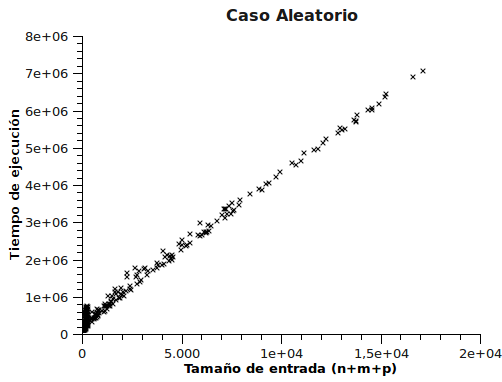
\includegraphics[scale=0.75]{img/ej3/CasoAleatorio.png} 
\end{center}

Al realizar una serie de casos de prueba para el peor caso, obtuvimos el siguiente gráfico del tiempo de ejecución en función del tamaño de la entrada: \\

\begin{center}
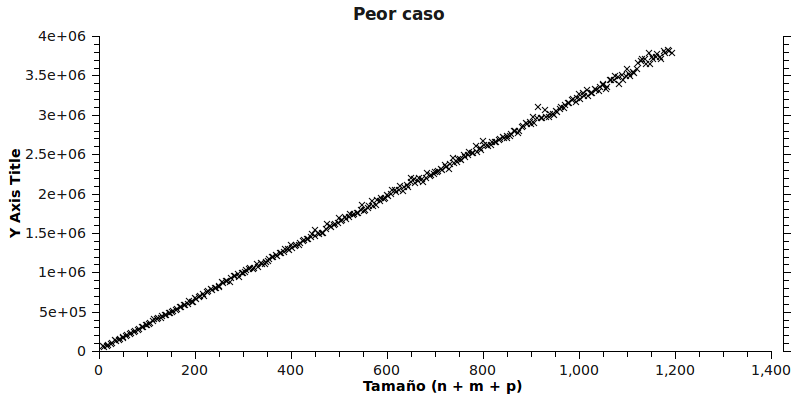
\includegraphics[scale=0.75]{img/ej3/peor_caso.png} 
\end{center}

Es importante aclarar que lo que terminamos graficando es el mínimo entre 3 mediciones de tiempo que tomamos para cada prueba. De esta forma tratamos de evitar outliers que puedan generarse por diversas razones (algoritmo de scheduling del sistema operativo, datos en la caché, etc.). \\
